%% ----------------------------------------------------------------
%% Article.tex
%% ---------------------------------------------------------------- 
\documentclass{ecsarticle}     % Use the Article Style
\graphicspath{{Figures/}}   % Location of your graphics files
\usepackage{natbib}            % Use Natbib style for the refs.
\hypersetup{colorlinks=false}   % Set to false for black/white printing
\input{Definitions}            % Include your abbreviations

\usepackage[nodayofweek]{datetime}
\usepackage{listings}
\usepackage{color}

\usepackage{graphicx}



%% ----------------------------------------------------------------
\begin{document}
%TC:ignore
\frontmatter
\title      {COMP6036: Advanced Machine Learning\\
            An investigation into DBSCAN}
      
\addresses  {\deptname\\\univname}
\authors                 {\href{mailto:ajr2g10@ecs.soton.ac.uk}{Ashley J. Robinson}\\\href{mailto:ajr2g10@ecs.soton.ac.uk}{ajr2g10@ecs.soton.ac.uk}}

\date       {\today}
\subject    {}
\keywords   {}
\maketitle
%% ----------------------------------------------------------------


\begin{abstract}
The paper chosen for the research report is entitled \textbf{A density-based algorithm for discovering clusters in large spatial databases with noise} which introduces the algorithm DBSCAN.
DBSCAN is used for clustering sparse spatial databases using data point density.
The algorithm performs well at this but has some shortcomings when applied to tasks which hold clusters of different densities.
Only one priori, cluster density, is required but this can be difficult to tune in high dimensional space.
The algorithm is compared against other common cluster implementations using a machine learning toolkit for Python.
\end{abstract}

%TC:endignore
\mainmatter


\section{Motivation for Algorithm}

DBSCAN (Density-Based Spatial Clustering of Applications with Noise) is an unsupervised application of machine learning introduced by~\cite{ester96dbscan}.
Intended to address Spatial Database Systems (SDBS) which can be produced from naturally occurring geometric and geographical datasets or applications such a layout for integrated circuit design~\citep{guting94sdbs}.
It has three main objectives.
To minimise the required domain knowledge needed to set input parameters, have the capability to discover clusters of arbitrary shapes and to perform well on large spatial databases.

At the time of creation the algorithms was compared to a recent development called CALARANS~\citep{ng94clarans} which is an extension of CLARA (Clustering LARge Applications)~\citep{kaufman90clara}.
Both algorithms are intended for use on large databases but CLARANS uses random noise to improve performance.
Apart from traditional clustering algorithms where first principles are introduced, such a K-means, DBSCAN was a breakthrough in terms of a density approach to datasets.

\section{Technical Explanation}

DBSCAN uses cluster density to classify data.
It is intuitive to build a community of data points by attempting to draw a path of connectivity between points.
This leads to the first input parameter to the algorithm, $\epsilon$, which is a threshold for the distance that DBSCAN is permitted to move yet remain in the same cluster.
Equation~\eqref{eqn:dist}, adapted from~\cite{ester96dbscan}, is the basic function used to determine membership by thresholding; euclidean distance is used in this case but the measure of distance can be replaced with a Manhattan norm to scale down computational overheads therefore favouring large datasets~\citep{krause86taxicab}.
Only two input patterns are compare at once and all belong to the set of training data, $\textbf{x}$, containing $n$ input patterns.

\begin{equation}
	N(\textbf{p},\textbf{q},\epsilon) = \left\{
		\begin{array}{l}
    		1,\: ||\textbf{p} - \textbf{q}|| \leq \epsilon\\
    		0,\: ||\textbf{p} - \textbf{q}|| > \epsilon
  		\end{array} \right.
	\:\:where\:\: \textbf{q},\textbf{p} \in \textbf{x}
	\label{eqn:dist}
\end{equation}


This approach is simple for compact clusters but when noise is introduced the algorithm will identify a few points as a whole cluster.
This is possibly down to a badly tuned value for $\epsilon$ but can be negated by introducing a second threshold to set the minimum number of members a cluster can have however this is unnecessary to perform basic DBSCAN clustering.
Equation~\eqref{eqn:member} takes the sum of connected data points attributed to a single point which used for the comparison in Equation~\eqref{eqn:inside}. 
The parameter, $\lambda$, if successfully applied to Equation~\eqref{eqn:inside} decides when to build a cluster around the point.

\begin{equation}
	C(\textbf{x}_i,\epsilon) =  \sum\limits_{j=1 \atop j\:\neq\:i}^n N(\textbf{x}_i,\textbf{x}_j,\epsilon)	
	\label{eqn:member}
\end{equation}

\begin{equation}
	\lambda \leq C(\textbf{p},\epsilon) 
	\label{eqn:inside}
\end{equation}

A low dimensional representation of the constraints used in DBSCAN is held in Figure~\ref{fig:circles} which contains seven points labelled \textbf{A} to \textbf{H}.
A string of points are density connected in the centre of the diagram, two points on the left and is \textbf{G} is unconnected.
Increasing $\epsilon$ will merge these three possible clusters.
Equation~\eqref{eqn:clusters} describes how possible values of $\lambda$ can change the clustering of Figure~\ref{fig:circles}.


\begin{figure}[ht]
   \centering
    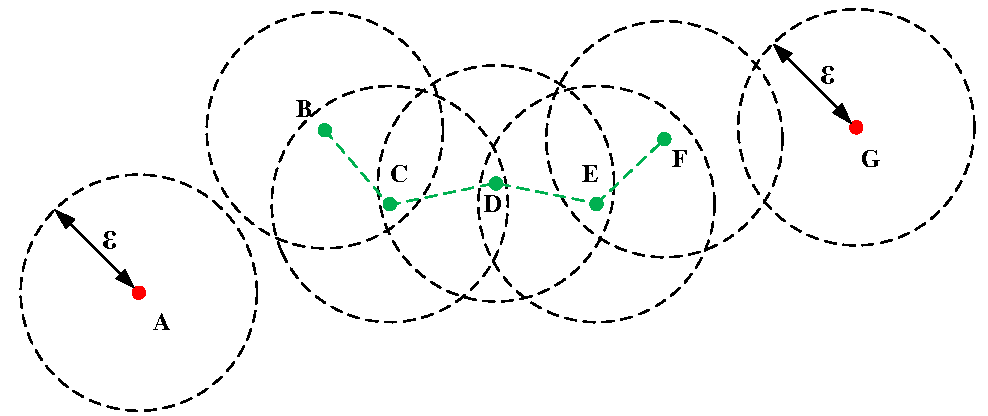
\includegraphics[height = 4cm]{circles.pdf}
   \caption{2D application of DBSCAN.}
   \label{fig:circles}
\end{figure}

\begin{equation}
	\# Clusters = \left\{
		\begin{array}{l}
    		0\:if\; \lambda \geq 6\\
    		1\:if\; \lambda = 5 \\
			2\:if\; 2 \leq \lambda \leq 5 \\
			3\:if\; \lambda = 1\\
  		\end{array} \right.
	\label{eqn:clusters}
\end{equation}




It is clear there is a lot of scope for optimisation in practice.
A list containing all datapoints at the start of the algorithm can be used to check off points which have been found to belong to a cluster.
This means for an input space containing $\alpha$ clusters that can be perfectly segmented by DBSCAN requires only $\alpha$ calls of Equation~\eqref{eqn:member}.
Formally a set of unclassified vectors, $\textbf{b} \in \textbf{x}$, can be defined and passed to Equation~\eqref{eqn:member} requiring much fewer evaluations. 


\section{Performance}

The graphs in Figure~\ref{fig:compare} are different clustering algorithms applied to a shape dataset taken from~\cite{gionis05cluster}.
Chosen for comparison is K-Means because it is arguably the most well-known clustering algorithm and WARD because of its performance on this dataset when compared against other available algorithms.
Implementations were taken from a machine learning toolbox for Python~\citep{scikit13ml}.
The dataset contains seven clusters but in two cases there are \emph{bridges} between the clusters.
On the far right K-Means and WARD correctly divides the data where DBSCAN incorrectly groups both clusters together; shown in Figures~\ref{fig:kmeans},~\ref{fig:ward} and~\ref{fig:dbscan} respectively.
DBSCAN deals well with the remaining data where the other two algorithms fail due to its ability to negate relatively tight clusters.

\begin{figure}[ht]
   \centering
   \subfigure[K-Means]{
      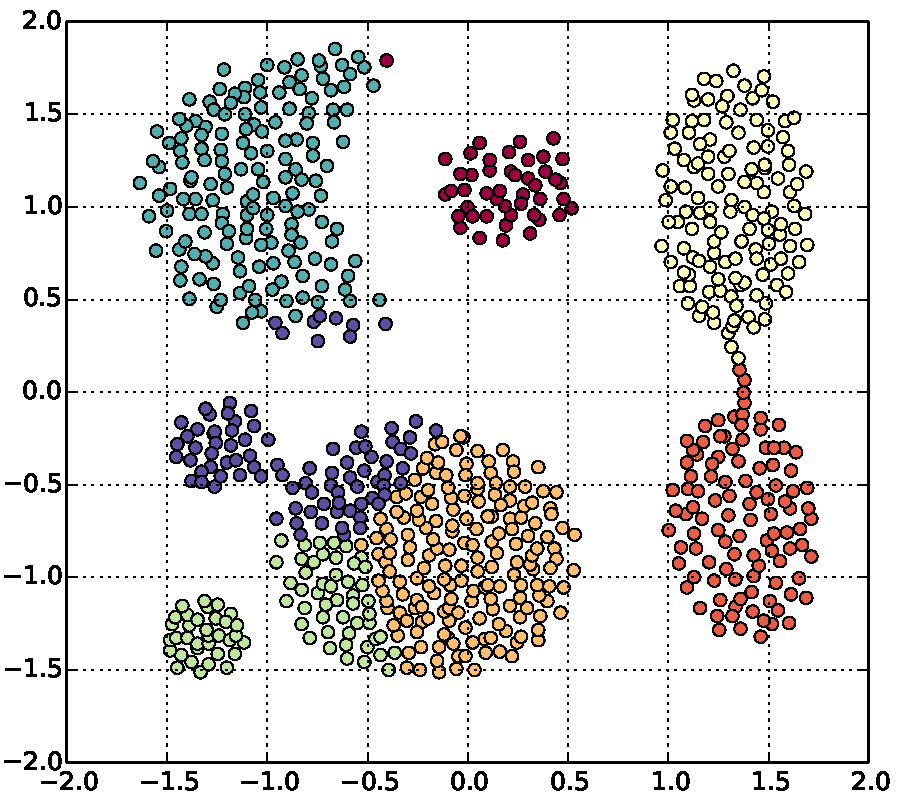
\includegraphics[height = 5cm,width = 5cm]{kmeans.pdf}
      \label{fig:kmeans}
   }
   \subfigure[WARD]{
      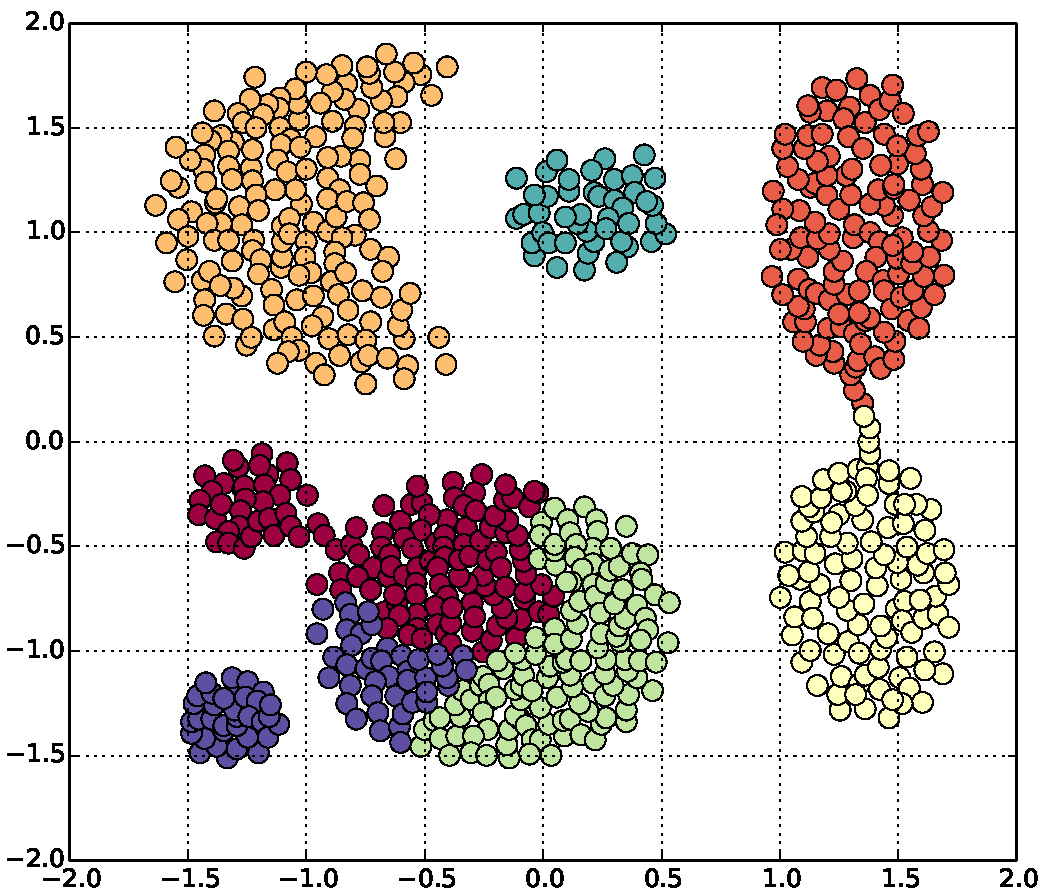
\includegraphics[height = 5cm, width = 5cm]{ward.pdf}
      \label{fig:ward}
   }
   \subfigure[DBSCAN]{
      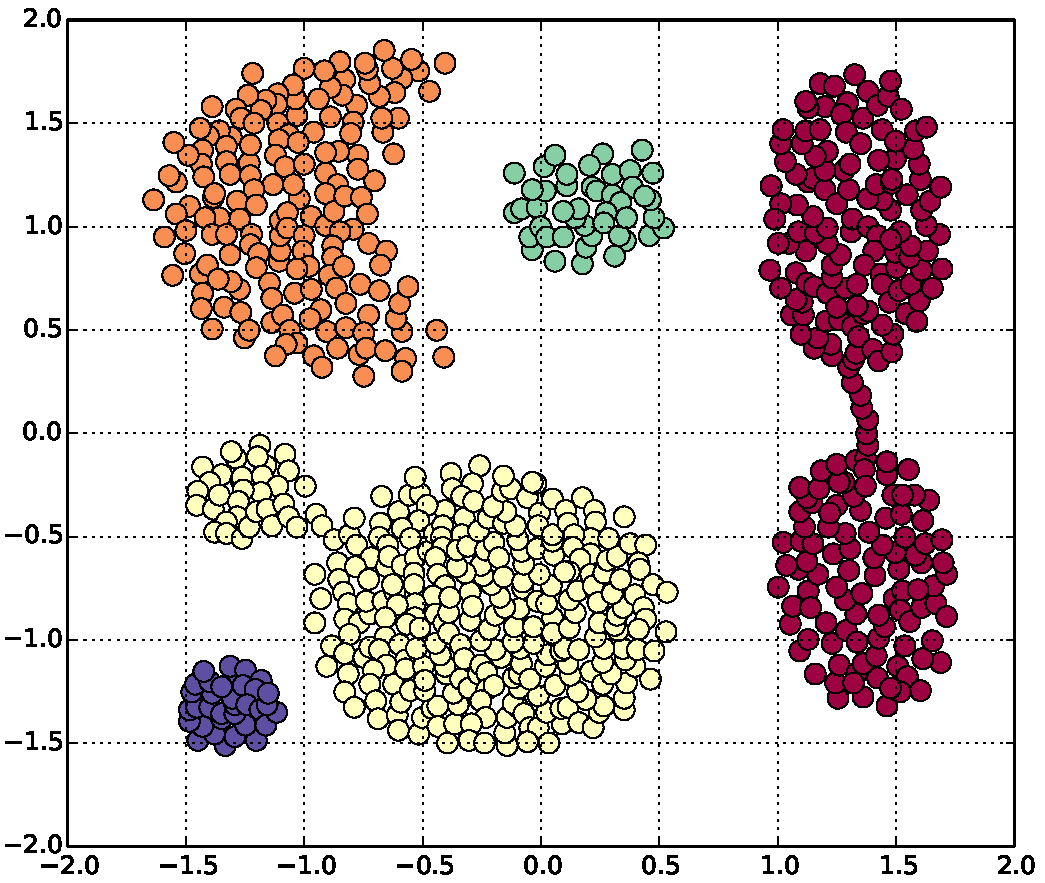
\includegraphics[height = 5cm,width = 5cm]{dbscan.pdf}
      \label{fig:dbscan}
   }
   \caption{A comparison against DBSCAN.}
   \label{fig:compare}
\end{figure}

The algorithm exhibits variation in performance as per the standard bias-variance dilemma.
Figure~\ref{fig:error} shows how the error varies for with $\epsilon$ when applied to data used in Figure~\ref{fig:compare}.
Objectively DBSCAN doesn't perform well on this dataset missing two clusters completely however this is crafted cornerstone case intended to trap algorithms.

\begin{figure}[ht]
   \centering
    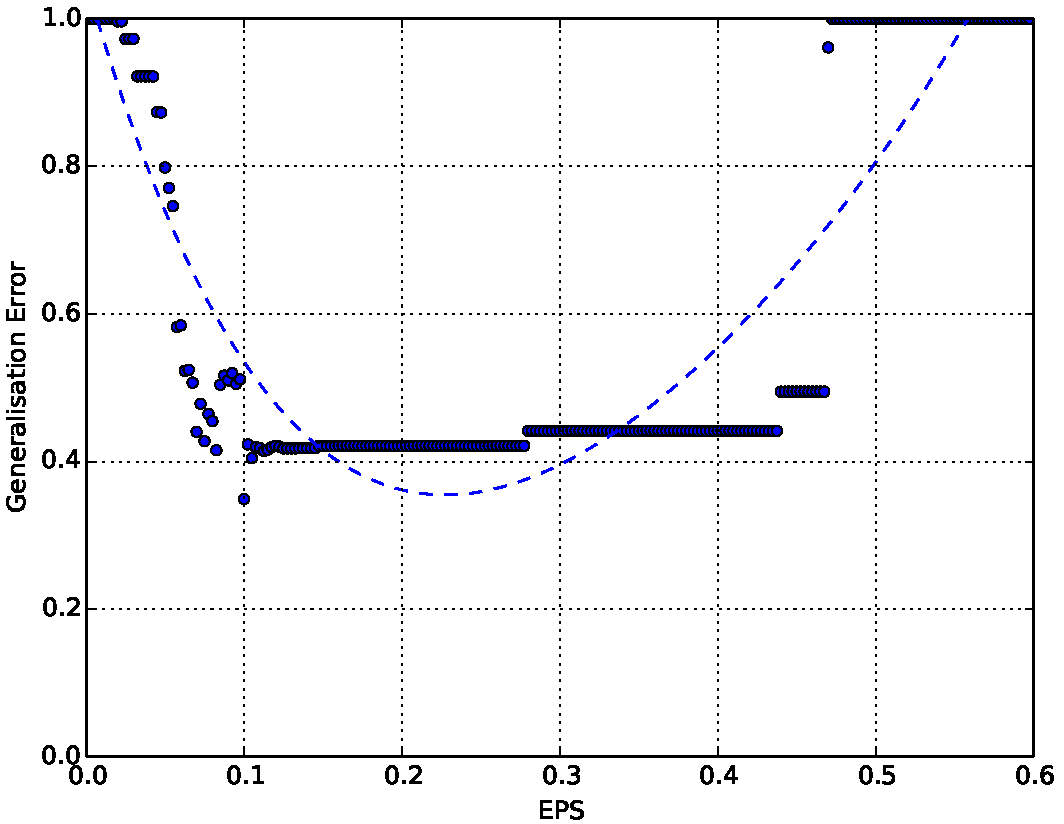
\includegraphics[height = 5cm,width = 8cm]{error.pdf}
   \caption{Generalisation error while varying the $\epsilon$ input parameter.}
   \label{fig:error}
\end{figure}




\section{Extensions}
Since the creation of this algorithm extension have been trialed . 

\cite{lian07ldbscan} considered the difficulty to select a value for $\epsilon$ and adapted the algorithm to LDBSCAN (Local-DBSCAN).

\section{Conclusions}
DBSCAN performs well on spatial database and can be optimised to be extremely efficient.
As per most unsupervised clustering algorithms this is particularly appealing for good results with using simple methods. 
There are downsides to algorithm

%TC:ignore
\bibliographystyle{ecs}
\bibliography{references}



\backmatter
\begin{appendix}

\newpage
\section{Code Listings}
\lstset{ %
     language=Python,                % the language of the code
  basicstyle=\footnotesize,           % the size of the fonts that are used for the code
  numbers=none,                   % where to put the line-numbers
  numberstyle=\tiny\color{black},  % the style that is used for the line-numbers
  stepnumber=2,                   % the step between two line-numbers. If it's 1, each line 
                                  % will be numbered
  numbersep=5pt,                  % how far the line-numbers are from the code
  backgroundcolor=\color{white},      % choose the background color. You must add \usepackage{color}
  showspaces=false,               % show spaces adding particular underscores
  showstringspaces=false,         % underline spaces within strings
  showtabs=false,                 % show tabs within strings adding particular underscores
  rulecolor=\color{black},        % if not set, the frame-color may be changed on line-breaks within not-black text (e.g. comments (green here))
  tabsize=2,                      % sets default tabsize to 2 spaces
  captionpos=b,                   % sets the caption-position to bottom
  breaklines=true,                % sets automatic line breaking
  breakatwhitespace=false,        % sets if automatic breaks should only happen at whitespace
  title=\lstname,                   % show the filename of files included with \lstinputlisting;
                                  % also try caption instead of title
  keywordstyle=\color{blue},          % keyword style
  commentstyle=\color{green},       % comment style
  stringstyle=\color{red},         % string literal style
  escapeinside={\%*}{*)},            % if you want to add LaTeX within your code
  morekeywords={*,...},              % if you want to add more keywords to the set
  deletekeywords={...}              % if you want to delete keywords from the given language
}

\lstinputlisting[caption=K-Means clustering.,label={KMEANS.py}]{../Code/KMEANS.py}
\newpage
\lstinputlisting[caption=WARD Clustering.,label={WARD.py}]{../Code/WARD.py}
\newpage
\lstinputlisting[caption=DBSCAN Clustering.,label={DBSCAN.py}]{../Code/DBSCAN.py}
\newpage
\lstinputlisting[caption=Tuning DBSCAN.,label={tuneDBSCAN}]{../Code/tuneDBSCAN.py}
\end{appendix}

%TC:endignore
\end{document}
%% ----------------------------------------------------------------

